% Guava Fruit Disease Classification (GFDD24) -- Beamer slides
% Engine: bin/tectonic (self-contained TeX). Compile: ../bin/tectonic slides.tex
\documentclass[aspectratio=169]{beamer}
\usetheme{Madrid}
\definecolor{navy}{HTML}{1B3B6F}
\definecolor{myblue}{HTML}{2E75B6}
\usecolortheme[named=navy]{structure}
\setbeamercolor{title}{bg=navy,fg=white}
\setbeamercolor{frametitle}{bg=navy!12,fg=navy}
\setbeamercolor{block title}{bg=myblue,fg=white}
\setbeamercolor{block body}{bg=myblue!8,fg=black}
\setbeamertemplate{itemize item}{\color{myblue}$\blacktriangleright$}
\setbeamertemplate{navigation symbols}{}
\setbeamertemplate{footline}{%
  \leavevmode\hbox{%
    \begin{beamercolorbox}[wd=.4\paperwidth,ht=2.4ex,dp=1ex,left]{author in head/foot}%
      \usebeamerfont{author in head/foot}\hspace{1ex}Nihar Ranjan Mishra, Aaviraj Nikumbh, Neel Lakhani%
    \end{beamercolorbox}%
    \begin{beamercolorbox}[wd=.4\paperwidth,ht=2.4ex,dp=1ex,center]{title in head/foot}%
      \usebeamerfont{title in head/foot}Guava Disease Classification (GFDD24)%
    \end{beamercolorbox}%
    \begin{beamercolorbox}[wd=.2\paperwidth,ht=2.4ex,dp=1ex,right]{date in head/foot}%
      \usebeamerfont{date in head/foot}\insertframenumber{} / \inserttotalframenumber{}\hspace{1ex}%
    \end{beamercolorbox}}%
}
\usepackage{graphicx}
\usepackage{booktabs}
\graphicspath{{../outputs/audit/}{../outputs/plots/}{../outputs/results/}}
\title{Guava Fruit Disease Classification}
\subtitle{Custom CNN from scratch vs.\ MobileNetV2 transfer learning (GFDD24)}
\author{Nihar Ranjan Mishra \and Aaviraj Nikumbh \and Neel Lakhani}
\institute{Course project --- seed 42 everywhere; CPU-only build (Apple Silicon, 224px)}
\date{October 2026}
\begin{document}
% 1 Title
\begin{frame}
  \titlepage
\end{frame}
% 2 Agenda
\begin{frame}{Agenda}
  \begin{itemize}
    \item Problem and motivation
    \item Related work: overview table (2.1), method families (2.2), gap (2.3)
    \item Dataset audit + leakage finding
    \item CNN and transfer-learning concepts; data pipeline
    \item Model A vs Model B; project structure and tools
    \item Results, confusion matrices, Grad-CAM
    \item Error analysis, limitations, conclusion, references
  \end{itemize}
\end{frame}
% 3 Problem
\begin{frame}{Problem and motivation}
  \begin{itemize}
    \item Classify guava fruit photos into \textbf{Anthracnose / Fruit Flies / Healthy} to enable early, automatic disease triage.
    \item \textbf{Model A}: custom 4-block CNN from scratch (1.24M params) vs.\ \textbf{Model B}: ImageNet-pretrained MobileNetV2 + head, then fine-tune last 30 layers.
    \item Released splits leak (same fruit in train and test) --- so we report \textbf{released and leak-free} accuracy side by side, plus Grad-CAM evidence.
    \item Headline (test, seed 42): A \textbf{0.911} / F1 0.917 vs.\ B \textbf{0.992} / F1 0.991.
  \end{itemize}
\end{frame}
% 4 Related work 2.1
\begin{frame}{Related work (2.1): comparative overview}
  \scriptsize
  \begin{tabular}{lllll}
    \toprule
    Study & Method & Data & Result & Limit \\
    \midrule
    Mostafa et al.\ 2021 & 5 CNNs, R-50 best & 321$\to$2889, 5 cl.\ & 99.54\% & other set, no ctl/XAI \\
    Doutoum et al.\ 2023 & Transfer, E-B3 & 1834 leaves, 5 cl.\ & 94.93\% & leaf-only, no XAI \\
    Nandi et al.\ 2022 & 5 CNNs + quant.\ & 681+8525, 5 cl.\ & 99\% / 97\% & mixed, no XAI \\
    Kilci \& Koklu 2024 & SqueezeNet+GB & GFDD24 3784 & 95.6\% & curated only \\
    Tewari et al.\ 2024 & DenseNet169 & 527, 5 cl.\ & 99.62\% & small, no XAI \\
    \bottomrule
  \end{tabular}
  \begin{itemize}
    \item Full 12-study table with verification URLs: \texttt{report/survey.md} \S8; BibTeX: \texttt{report/references.bib}. Pratama 2025 dropped (unverifiable).
  \end{itemize}
\end{frame}
% 5 Related work 2.1 cont + 2.2
\begin{frame}{Related work (2.1 cont.\ / 2.2): families}
  \scriptsize
  \begin{tabular}{lllll}
    \toprule
    Study & Method & Data & Result & Limit \\
    \midrule
    Zhou 2026 & VGG16+MNetV2+Grad-CAM & 527, 5 cl.\ & 96\% & other taxonomy \\
    ResNet-101 2025 & Transfer+XAI & GFDD24 & 98.48\% & curated only \\
    CNN-GB ens.\ 2025 & EffNet-B0+XGB & GFDD24 & $\sim$99.99\%* & preprint, leaked \\
    Mohanty 2016 & Alex/GoogLeNet & PlantVillage 54k & 99.35\% & lab-field gap \\
    \bottomrule
  \end{tabular}
  \begin{block}{Method families (2.2)}
    \footnotesize Transfer architectures (ours B) \quad / \quad hybrid deep-features+boosting \quad / \quad data-centric (aug-before-split, quant., CLAHE).
  \end{block}
\end{frame}
% 6 Related work 2.3 gap
\begin{frame}{Related work (2.3): gap and positioning}
  \begin{block}{Defensible gap}
    No verified GFDD24 study reports \textbf{(i)} from-scratch vs two-phase transfer head-to-head, \textbf{(ii)} with duplicate quantification, \textbf{(iii)} a leak-free control, \textbf{(iv)} Grad-CAM on the same split. [5,8,9] report GFDD24 accuracy (95.6--99.99\%) on the leaked split without controls.
  \end{block}
  \begin{itemize}
    \item We do not claim ``no MobileNetV2 on guava'' ([4,7] did). Claim softens to ``among the first'' if a 4-part study surfaces --- table gives everything to check.
  \end{itemize}
\end{frame}
% 7 Dataset
\begin{frame}{Dataset (GFDD24, Mendeley DOI 10.17632/bkdkc4n835.1)}
  \begin{itemize}
    \item 473 field originals (Rajshahi/Pabna, July, pathologist-verified), unsharp+CLAHE to 512x512 RGB PNG, augmented x8 to \textbf{3,784 images}.
    \item On disk: train 2647 (1080 / 918 / 649), val \textbf{755} (308 / 262 / 185), test 382 (156 / 132 / 94).
    \item Release notes say val 775 --- \textbf{20-image shortfall reported, not hidden}.
    \item All 3,784 decode clean (0 corrupt); folders read from disk: Anthracnose, fruit\_fly, healthy\_guava.
  \end{itemize}
\end{frame}
% 8 CNN concepts
\begin{frame}{Concepts: CNN classifier}
  \begin{itemize}
    \item Conv $3\times3$ learns local lesion/puncture textures; stacked blocks (32/64/128/256) build scale; MaxPool halves resolution; GAP averages to 256-d.
    \item BatchNorm stabilizes layer inputs (Ioffe \& Szegedy 2015); Dropout 0.25/0.5 breaks co-adaptation (Srivastava et al.\ 2014).
    \item Softmax + categorical cross-entropy; Adam 1e-3 (Kingma \& Ba 2015). Fix found here: BN momentum 0.9 (not 0.99) so moving averages track fast-learning small-data stats.
  \end{itemize}
\end{frame}
% 9 Transfer concepts
\begin{frame}{Concepts: two-phase transfer learning}
  \begin{itemize}
    \item Yosinski et al.\ 2014: early filters (edges/blobs) transfer; late layers specialize. ImageNet (Deng et al.\ 2009) is the source.
    \item Phase 1 (head warm-up): backbone frozen incl.\ BatchNorm, lr 1e-3, 15 epochs. Phase 2: unfreeze last 30 layers, BN kept frozen, lr 1e-5, 20 epochs.
    \item MobileNetV2 (Sandler et al.\ 2018): inverted residuals + linear bottlenecks; inputs mapped $[0,1]\to[-1,1]$ via Rescaling (no Lambda, safe .keras reload).
  \end{itemize}
\end{frame}
% 10 Pipeline
\begin{frame}{Data pipeline}
  \begin{itemize}
    \item \texttt{image\_dataset\_from\_directory}, categorical labels, class order from disk, seed 42, shuffle train only; rescale $[0,1]$; prefetch.
    \item Train-only augmentation: flip H+V, rotation 0.15, zoom 0.15, contrast 0.1, brightness 0.1 (value\_range fixed to $(0,1)$ --- default $(0,255)$ blew train to 24).
    \item 224px CPU fallback (native 512px); batch 32; single seed 42 (stated scope cut).
  \end{itemize}
\end{frame}
% 11 Architectures
\begin{frame}{Model A vs Model B}
  \begin{columns}
    \begin{column}{0.5\textwidth}
      \textbf{A: custom CNN (1,243,683 params)}
      \begin{itemize}
        \item 4$\times$[Conv-ReLU-BN x2, Pool, Drop 0.25]; GAP; Dense256-ReLU-BN-Drop0.5; softmax. Adam 1e-3, $\le$40 ep.
      \end{itemize}
    \end{column}
    \begin{column}{0.5\textwidth}
      \textbf{B: MobileNetV2 TL (2,586,691)}
      \begin{itemize}
        \item Frozen backbone + Dense256-Drop0.4 head; FT last 30 (BN frozen). 1e-3/15 + 1e-5/20.
      \end{itemize}
    \end{column}
  \end{columns}
  \begin{itemize}
    \item Shared: CCE, ES (val\_loss, patience 8, restore best), ReduceLROnPlateau, best-val\_acc checkpoint, save/reload parity True.
  \end{itemize}
\end{frame}
% 12 Structure
\begin{frame}{Project structure and tools}
  \begin{itemize}
    \item \texttt{config.py data\_pipeline.py models.py train.py evaluate.py scripts/\{audit,gradcam,make\_figures\}.py}
    \item \texttt{Dataset/ Dataset\_leakfree/ outputs/\{models,logs,plots,audit,results\}/ report/}
    \item Tools: TF 2.21 CPU, sklearn, matplotlib/seaborn, imagehash, Tectonic Beamer. One command per stage in README.
  \end{itemize}
\end{frame}
% 13 Results
\begin{frame}{Results (test 382, seed 42) --- every number from executed runs}
  \footnotesize
  \begin{tabular}{lcccc}
    \toprule
    Model & Test & Macro F1 & Val & Time \\
    \midrule
    A: Custom CNN & 0.9110 & 0.9173 & 0.9364 & 31.6 min \\
    B: MobileNetV2 TL & 0.9921 & 0.9911 & 0.9960 & 14.5 min \\
    B frozen (no FT) & 0.9948 & 0.9942 & 0.9907 & 6.2 min \\
    B no-augment & 0.9948 & 0.9946 & 0.9974 & 13.1 min \\
    \bottomrule
  \end{tabular}
  \begin{itemize}
    \item B beats A by $\sim$8pp; frozen/noaug match full B on leaked split (head suffices; release aug covers variation). Leak-free: A-control 0.9923 (partial ckpt), B-control 0.9872 --- no visible inflation (task saturates).
  \end{itemize}
\end{frame}
% 14 CM + GradCAM
\begin{frame}{Confusion matrices and Grad-CAM}
  \begin{columns}
    \begin{column}{0.5\textwidth}
      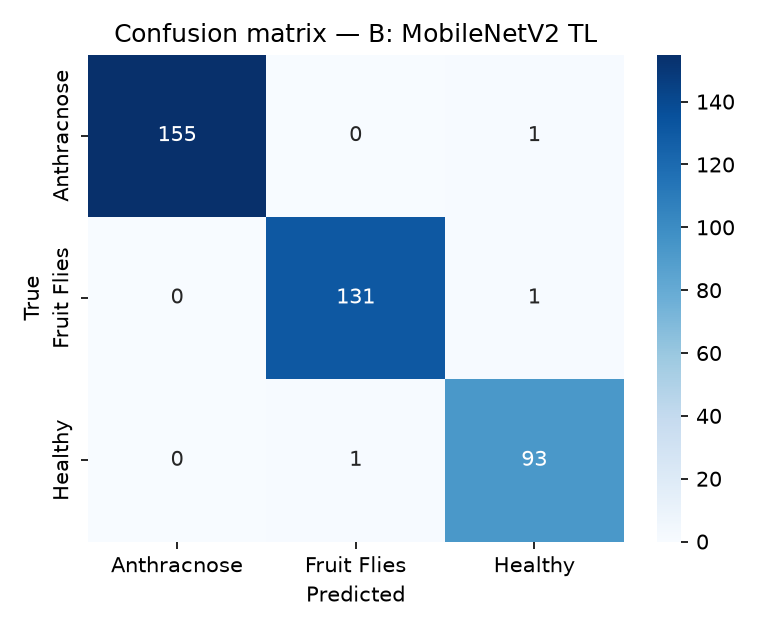
\includegraphics[width=\linewidth]{../outputs/plots/transfer_MobileNetV2_base_cm.png}
    \end{column}
    \begin{column}{0.5\textwidth}
      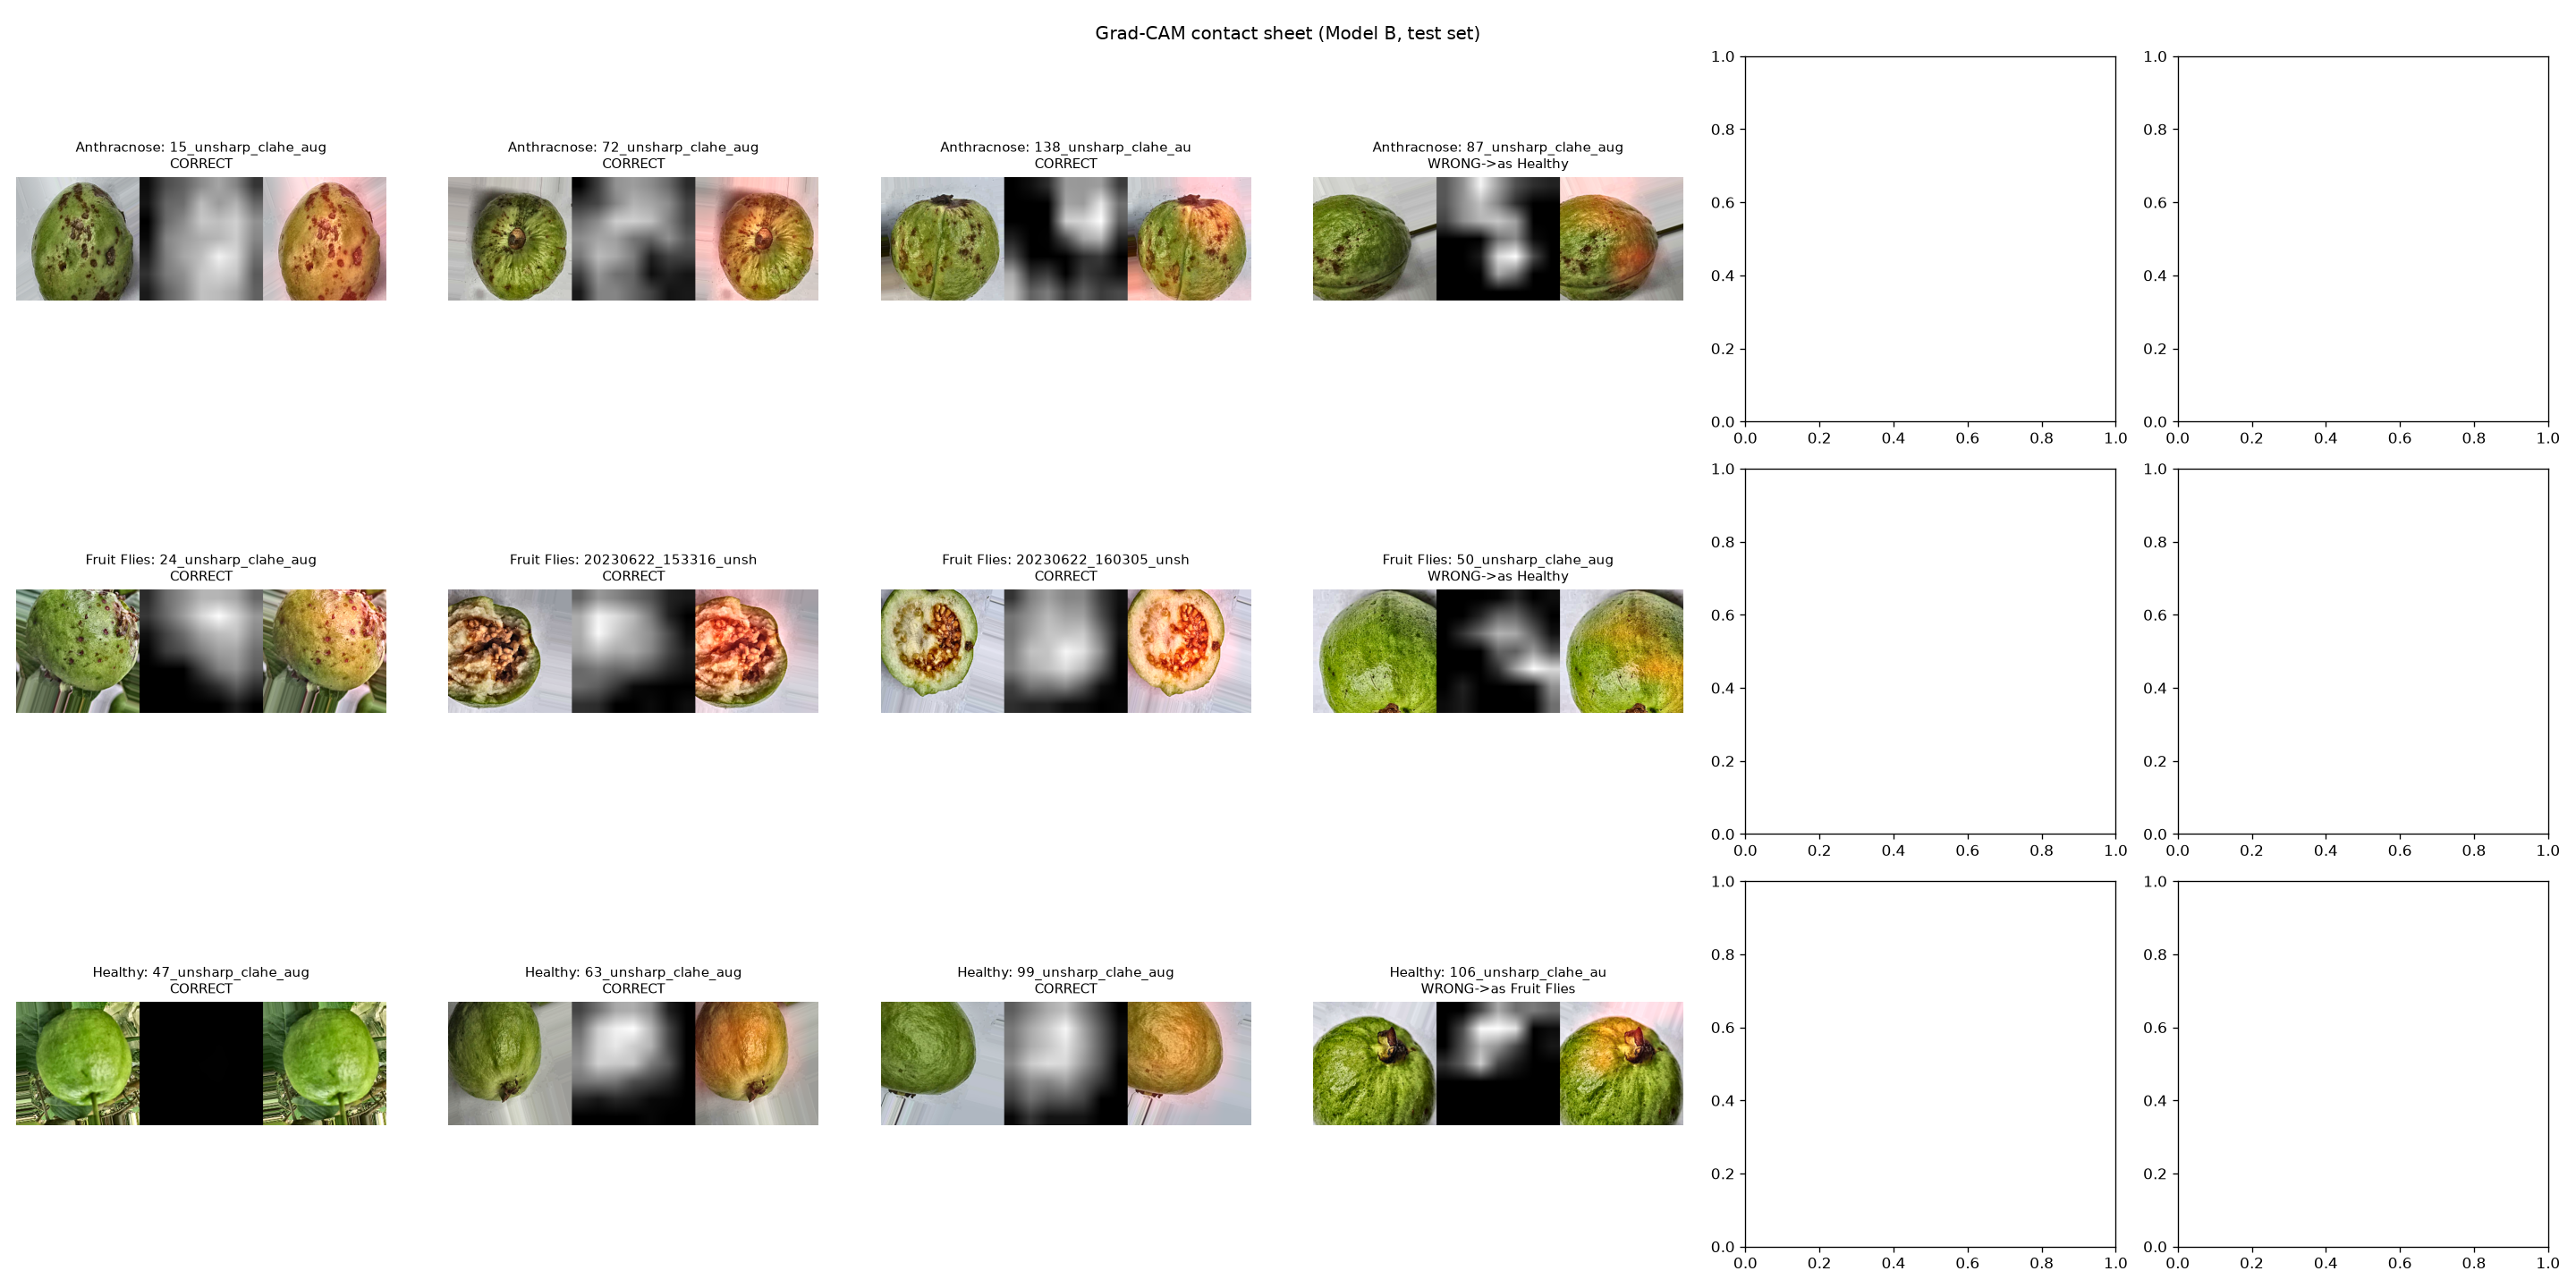
\includegraphics[width=\linewidth]{../outputs/plots/gradcam_contact_sheet.png}
    \end{column}
  \end{columns}
  \begin{itemize}
    \item B: 3 errors total. A: 26 Anthracnose$\to$Fruit-Flies. Grad-CAM (Selvaraju et al.\ IJCV 2020) on deepest backbone conv: lesions/punctures highlighted, not background.
  \end{itemize}
\end{frame}
% 15 Error + limits
\begin{frame}{Error analysis and limitations}
  \begin{itemize}
    \item Confusable pair: Anthracnose lesions vs fruit-fly punctures (dark spots). Curves: A wobbles (val 0.93$\to$0.71$\to$0.94, ES kept ep8); B tracks cleanly.
    \item Leakage: 454/473 originals span splits; 100\% val/test share an original with train --- released scores are near-duplicate recognition (Tampu precedent). Control reported alongside.
    \item Limits: single seed 42; 224px fallback; val 755 vs 775; leakfree-custom ckpt interrupted 17/40 (best kept, stated).
  \end{itemize}
\end{frame}
% 16 Conclusion
\begin{frame}{Conclusion and future work}
  \begin{itemize}
    \item Transfer (B, 0.992) beats from-scratch (A, 0.911) on 2.6k images, faster (14.5 vs 31.6 min) and stabler. Frozen head alone already 0.995 on leaked split.
    \item Honest reporting (leakage quantified + control + Grad-CAM) matters more than the last point of accuracy.
    \item Future: field photos from new orchards; 512px + multi-seed; EfficientNetB0/ResNet50 backbones (already supported); deployment-size quantization (Nandi precedent).
  \end{itemize}
\end{frame}
% 17 References
\begin{frame}{References}
  \footnotesize
  \begin{itemize}
    \item [1] Al Amin et al.\ GFDD24, Mendeley Data 2024, DOI 10.17632/bkdkc4n835.1.
    \item [2] Mostafa et al.\ Appl.\ Sci.\ 12(1):239, 2021. [3] Doutoum et al.\ WSEAS 20:356-363, 2023. [4] Nandi et al.\ MIET/arXiv:2209.12557, 2022.
    \item [5] Kilci \& Koklu, Proc.\ FIAR 2024. [6] Mohanty et al.\ Front.\ Plant Sci.\ 2016. [7] Sandler et al.\ CVPR 2018.
    \item [8] Tampu et al.\ Sci.\ Data 9:580, 2022. [9] Selvaraju et al.\ IJCV 2020. [10] Kingma \& Ba ICLR 2015; Ioffe \& Szegedy ICML 2015; Yosinski et al.\ NeurIPS 2014. Full 22-entry BibTeX: \texttt{report/references.bib}.
  \end{itemize}
\end{frame}
% 18 Thank you
\begin{frame}
  \centering
  {\Large Thank you}\\[1ex]
  Nihar Ranjan Mishra, Aaviraj Nikumbh, Neel Lakhani\\[1ex]
  Code, results, and slides fully reproducible from \texttt{README.md} (seed 42).
\end{frame}
\end{document}
